\chapter{Elettronica combinatoria complessa}
\label{ch:comb-complessa}
\textit{(11 maggio 2026)}

\noindent Si tratta di circuiti combinatori ``di alto livello'' che permettono di
implementare funzioni logiche in modo compatto e regolare, senza progettare ogni volta una
rete di porte su misura: le \textbf{memorie ROM}, le \textbf{PLA}, i \textbf{multiplexer} e
i \textbf{demultiplexer}. Alla fine del capitolo questi blocchi vengono combinati con i
flip-flop per costruire il \textbf{registro a scorrimento universale} (USR).

% ======================================================================
\section{ROM -- Read Only Memory}

\begin{definizione}{ROM}
\textbf{ROM} (\emph{Read Only Memory}): circuito con $n$ linee di ingresso (indirizzo) e $p$
linee di uscita. Con $n$ linee di ingresso si hanno $2^n$ possibili combinazioni, e a
ciascuna la ROM associa una parola di $p$ bit. Può essere interpretata in 2 modi:
\begin{enumerate}[leftmargin=1.5em]
    \item \textbf{memoria} da $2^n$ parole da $p$ bit: l'ingresso è l'\emph{indirizzo}, l'uscita
          è il \emph{contenuto} della cella indirizzata;
    \item \textbf{implementazione di $p$ funzioni} delle $n$ variabili in ingresso: ogni
          colonna di uscita è la tabella di verità di una funzione.
\end{enumerate}
\end{definizione}

\begin{center}
\begin{tikzpicture}[font=\small, >=latex, line width=0.6pt]
\node[draw, thick, minimum width=2cm, minimum height=1.4cm, fill=noteblue!4] (rom) {ROM};
\draw[->, very thick] ($(rom.west)+(-1.4,0)$) -- node[above] {$n$} (rom.west);
\draw[->, very thick] (rom.east) -- node[above] {$p$} ++(1.4,0);
\foreach \x in {-0.7}{ \draw ($(rom.west)+(\x-0.08,-0.14)$) -- ++(0.16,0.28); }
\draw ($(rom.east)+(0.62,-0.14)$) -- ++(0.16,0.28);
\node[below, font=\scriptsize] at ($(rom.west)+(-0.7,-0.2)$) {indirizzo};
\node[below, font=\scriptsize] at ($(rom.east)+(0.7,-0.2)$) {parola};
\end{tikzpicture}
\end{center}

\subsection{Come è fatta?}

Internamente la ROM è costituita da due blocchi in cascata:

\begin{center}
\begin{tikzpicture}[font=\small, >=latex, line width=0.6pt,
  blocco/.style={draw, thick, minimum width=2.4cm, minimum height=1.2cm, align=center, fill=noteblue!4}]
\node[blocco] (dec) at (0,0)   {decoder\\\scriptsize(piano AND)};
\node[blocco] (enc) at (4.6,0) {encoder\\\scriptsize(piano OR)};
\draw[->, very thick] (-2.4,0) -- node[above] {$n$} (dec.west);
\draw[->, very thick] (dec.east) -- node[above] {$2^n$} (enc.west);
\draw[->, very thick] (enc.east) -- node[above] {$p$} ++(1.4,0);
\node[below=3pt, font=\scriptsize, align=center] at (dec.south) {associa a un indirizzo\\una singola linea attiva};
\node[below=3pt, font=\scriptsize, align=center] at (enc.south) {associa a quella linea\\una parola in codice};
\end{tikzpicture}
\end{center}

\begin{itemize}[leftmargin=1.5em, itemsep=2pt]
    \item Il \textbf{decoder} (piano di AND e NOT) genera tutti i $2^n$ \textbf{mintermini} degli
          ingressi: per ogni indirizzo è attiva (a 1) una e una sola delle $2^n$ linee.
    \item L'\textbf{encoder} (piano di OR) trasforma la linea attiva nella parola di $p$ bit.
          Ogni uscita è l'OR dei mintermini per cui deve valere 1, cioè la funzione scritta in
          forma canonica SOP.
\end{itemize}

\noindent Per realizzare il piano di OR si usa una \textbf{matrice di diodi}: le linee dei
mintermini (orizzontali) incrociano le linee di uscita (verticali), ciascuna collegata a massa
tramite un resistore di \emph{pull-down}. Gli incroci di per sé non sono collegati; dove
l'uscita deve valere 1 si inserisce un diodo fra la riga e la colonna.

\medskip
\noindent Come esempio consideriamo una ROM con $n=2$ ingressi ($a_1a_0$) e $p=3$ uscite
($b_2b_1b_0$), cioè una memoria da 4 parole da 3 bit, con il contenuto seguente:

\begin{center}
\begin{tabular}{cc|c|ccc}
\toprule
$a_1$ & $a_0$ & mintermine & $b_2$ & $b_1$ & $b_0$ \\
\midrule
0 & 0 & $m_0=\overline{a_1}\,\overline{a_0}$ & 1 & 0 & 1 \\
0 & 1 & $m_1=\overline{a_1}\,a_0$ & 0 & 1 & 1 \\
1 & 0 & $m_2=a_1\,\overline{a_0}$ & 1 & 1 & 0 \\
1 & 1 & $m_3=a_1\,a_0$ & 0 & 0 & 1 \\
\bottomrule
\end{tabular}
\qquad
$\begin{aligned}
b_2 &= m_0 + m_2 \\
b_1 &= m_1 + m_2 \\
b_0 &= m_0 + m_1 + m_3
\end{aligned}$
\end{center}

\begin{fitcenter}
\begin{circuitikz}[line width=0.6pt, font=\small, >=latex]
\ctikzset{diodes/scale=0.45, resistors/scale=0.5}
% ingressi e loro negati (linee verticali)
\draw (0,5.0) node[above] {$a_1$} -- (0,-0.3);
\node[not port, rotate=-90, scale=0.6] (N1) at (0.7,4.4) {};
\draw (0,4.9) -| (N1.in 1);
\draw (N1.out) -- (0.7,-0.3);
\draw (1.6,5.0) node[above] {$a_0$} -- (1.6,-0.3);
\node[not port, rotate=-90, scale=0.6] (N0) at (2.3,4.4) {};
\draw (1.6,4.9) -| (N0.in 1);
\draw (N0.out) -- (2.3,-0.3);
\node[circle, fill, inner sep=1pt] at (0,4.9) {};
\node[circle, fill, inner sep=1pt] at (1.6,4.9) {};
% porte AND dei mintermini: righe y = 3,2,1,0
\foreach \k/\y/\xa/\xb in {0/3.2/0.7/2.3, 1/2.2/0.7/1.6, 2/1.2/0/2.3, 3/0.2/0/1.6}{
  \node[and port, scale=0.7] (A\k) at (3.6,\y) {};
  \draw (\xa,0 |- A\k.in 1) node[circle, fill, inner sep=1pt] {} -- (A\k.in 1);
  \draw (\xb,0 |- A\k.in 2) node[circle, fill, inner sep=1pt] {} -- (A\k.in 2);
  \draw (A\k.out) -- (8.6,\y) node[right, font=\scriptsize] {$m_\k$};
}
% colonne di uscita con pull-down
\foreach \c/\x in {2/5.4, 1/6.5, 0/7.6}{
  \draw (\x,-0.9) to[R] (\x,-1.9) node[ground] {};
  \draw (\x,-0.9) -- (\x,3.7);
  \draw[->] (\x,3.7) -- (\x,4.3) node[above, font=\scriptsize] {$b_\c$};
}
% diodi: dalla riga (anodo) alla colonna (catodo)
\foreach \x/\y in {5.4/3.2, 5.4/1.2, 6.5/2.2, 6.5/1.2, 7.6/3.2, 7.6/2.2, 7.6/0.2}{
  \draw (\x-0.45,\y) node[circle, fill, inner sep=1pt] {} to[D] (\x-0.45,\y-0.5) -- (\x,\y-0.5)
        node[circle, fill, inner sep=1pt] {};
}
\node[font=\footnotesize\bfseries, color=noteblue] at (1.8,-1.3) {piano AND e NOT (decoder)};
\node[font=\footnotesize\bfseries, color=noteblue] at (6.5,-3.1) {matrice di diodi (piano OR)};
\end{circuitikz}
\end{fitcenter}

\noindent\textbf{Funzionamento della matrice.} Quando un mintermine vale 1, la sua riga è a
livello alto e, attraverso i diodi presenti su quella riga, porta a 1 le colonne
corrispondenti; le colonne senza diodo restano a 0 grazie al pull-down. Se più righe sono
collegate alla stessa colonna, basta che una sola sia alta: la colonna realizza l'OR delle
righe (\emph{wired-OR}).

\begin{osservazione}{Perché diodi e non semplici collegamenti o resistenze}
Il diodo conduce solo dalla riga verso la colonna. Una colonna portata a 1 da una riga attiva
non può quindi ``rientrare'' in un'altra riga, che è a 0, attraverso un altro diodo
(polarizzato inversamente): le linee non si influenzano fra loro. Con un cortocircuito o con
delle resistenze, invece, le righe attive e inattive sarebbero collegate fra loro e i livelli
logici si mescolerebbero.
\end{osservazione}

\noindent Il circuito che implementa la ROM è quindi: \textbf{ROM = decoder + encoder}.

% ======================================================================
\subsection{Esempio: la tastiera}

Una tastiera numerica ha 10 tasti $T_0\ldots T_9$; a ogni tasto si associa il suo
\textbf{codice BCD} su 4 bit $B_3B_2B_1B_0$. Quando si preme un tasto, la sua linea viene
collegata a $+5$\,V; si ottiene così direttamente la ``linea singola attiva'' e basta il solo
encoder (matrice di diodi).

\begin{center}
\small
\begin{tabular}{c|cccc}
\toprule
Tasto & $B_3$ & $B_2$ & $B_1$ & $B_0$ \\
\midrule
$T_0$ & 0 & 0 & 0 & 0 \\
$T_1$ & 0 & 0 & 0 & 1 \\
$T_2$ & 0 & 0 & 1 & 0 \\
$T_3$ & 0 & 0 & 1 & 1 \\
$T_4$ & 0 & 1 & 0 & 0 \\
\bottomrule
\end{tabular}
\qquad
\begin{tabular}{c|cccc}
\toprule
Tasto & $B_3$ & $B_2$ & $B_1$ & $B_0$ \\
\midrule
$T_5$ & 0 & 1 & 0 & 1 \\
$T_6$ & 0 & 1 & 1 & 0 \\
$T_7$ & 0 & 1 & 1 & 1 \\
$T_8$ & 1 & 0 & 0 & 0 \\
$T_9$ & 1 & 0 & 0 & 1 \\
\bottomrule
\end{tabular}
\end{center}

\noindent Ogni uscita è l'OR delle righe (tasti) collegate alla sua colonna tramite un diodo:
\[
B_0 = T_1 + T_3 + T_5 + T_7 + T_9 \qquad
B_1 = T_2 + T_3 + T_6 + T_7 \qquad
B_2 = T_4 + T_5 + T_6 + T_7 \qquad
B_3 = T_8 + T_9
\]

\begin{fitcenter}
\begin{circuitikz}[line width=0.6pt, font=\small, >=latex]
\ctikzset{diodes/scale=0.4, resistors/scale=0.5}
\draw (0,5.3) node[left] {$+5$\,V} -- (0,0.5);
\foreach \t in {0,...,9}{
  \pgfmathsetmacro{\y}{5-0.5*\t}
  \draw (0,\y) node[circle, fill, inner sep=1pt] {} -- (0.3,\y) to[push button] (1.3,\y) -- (6.2,\y)
        node[right, font=\scriptsize] {$T_{\t}$};
}
\foreach \b/\x in {3/2.4, 2/3.4, 1/4.4, 0/5.4}{
  \draw (\x,5.2) -- (\x,-0.2) to[R] (\x,-1.2) node[ground] {};
  \draw[->] (\x,5.2) -- (\x,5.8) node[above, font=\scriptsize] {$B_\b$};
}
% diodi secondo il codice BCD
\foreach \t/\x in {1/5.4, 3/5.4, 5/5.4, 7/5.4, 9/5.4,
                   2/4.4, 3/4.4, 6/4.4, 7/4.4,
                   4/3.4, 5/3.4, 6/3.4, 7/3.4,
                   8/2.4, 9/2.4}{
  \pgfmathsetmacro{\y}{5-0.5*\t}
  \draw (\x-0.35,\y) node[circle, fill, inner sep=0.8pt] {} to[D] (\x-0.35,\y-0.3) -- (\x,\y-0.3)
        node[circle, fill, inner sep=0.8pt] {};
}
\end{circuitikz}
\end{fitcenter}

\noindent Si osservi che il tasto $T_0$ produce il codice 0000, identico alla condizione
``nessun tasto premuto'': nelle tastiere reali si aggiunge quindi un'uscita di
\emph{validità} (ad esempio l'OR di tutte le righe) che segnala la pressione di un tasto.

% ======================================================================
\subsection{Esempio: la ROM di un semaforo}

Una ROM può sostituire tutta la logica combinatoria di una macchina a stati finiti. Nel
semaforo gli ingressi della ROM sono lo stato presente $Q_1Q_0$ (memorizzato in due flip-flop
D) e un ingresso di abilitazione $E$; le uscite sono lo stato futuro $D_1D_0$, che torna ai
flip-flop, e i comandi delle tre lampade $V$ (verde), $G$ (giallo) e $R$ (rosso).

\begin{center}
\begin{tikzpicture}[font=\small, >=latex, line width=0.6pt,
  blocco/.style={draw, thick, align=center, fill=noteblue!4}]
\node[blocco, minimum width=1.8cm, minimum height=2.6cm] (rom) at (0,0) {ROM\\[2pt]\scriptsize $2^3$ parole\\\scriptsize da 5 bit};
\node[blocco, minimum width=1.6cm, minimum height=1.4cm] (ff) at (-3.4,0.2) {2 DFF};
\draw[->] (-5.4,-0.9) node[left] {$E$} -- ($(rom.west)+(0,-0.9)$);
\draw[->] ($(ff.east)+(0,0.3)$) -- node[above, font=\scriptsize] {$Q_1$} ($(rom.west)+(0,0.5)$);
\draw[->] ($(ff.east)+(0,-0.3)$) -- node[below, font=\scriptsize] {$Q_0$} ($(rom.west)+(0,-0.1)$);
\draw[->] ($(rom.east)+(0,0.9)$) -- ++(0.5,0) |- (-1.2,1.9) node[above, font=\scriptsize, pos=0.75] {$D_1$, $D_0$ (stato futuro)} -| (ff.north);
\foreach \o/\y in {V/0.2, G/-0.4, R/-1.0}{
  \draw[->] ($(rom.east)+(0,\y)$) -- ++(1.2,0) node[right] {$\o$};
}
\draw[<-] (ff.south) -- ++(0,-0.7) node[below, font=\scriptsize] {CLK};
\end{tikzpicture}
\end{center}

\noindent La ROM ha $n=3$ ingressi ($Q_1Q_0E$) e $p=5$ uscite ($D_1D_0VGR$): si programma
scrivendo, per ciascuno degli 8 indirizzi, lo stato futuro e le lampade da accendere.
Ad esempio, con $E=1$ il ciclo normale rosso $\to$ verde $\to$ giallo $\to$ rosso, e con
$E=0$ il giallo lampeggiante:

\begin{center}
\small
\begin{tabular}{cc|c|cc|ccc|l}
\toprule
$Q_1$ & $Q_0$ & $E$ & $D_1$ & $D_0$ & $V$ & $G$ & $R$ & significato \\
\midrule
0 & 0 & 1 & 0 & 1 & 0 & 0 & 1 & rosso, poi verde \\
0 & 1 & 1 & 1 & 0 & 1 & 0 & 0 & verde, poi giallo \\
1 & 0 & 1 & 0 & 0 & 0 & 1 & 0 & giallo, poi rosso \\
1 & 1 & 1 & 0 & 0 & 0 & 0 & 0 & spento, poi rosso \\
\midrule
0 & 0 & 0 & 1 & 1 & 0 & 0 & 1 & rosso, poi spento \\
0 & 1 & 0 & 1 & 1 & 1 & 0 & 0 & verde, poi spento \\
1 & 0 & 0 & 1 & 1 & 0 & 1 & 0 & giallo, poi spento \\
1 & 1 & 0 & 1 & 0 & 0 & 0 & 0 & spento, poi giallo \\
\bottomrule
\end{tabular}
\end{center}

\noindent Cambiare il comportamento del semaforo significa soltanto riprogrammare il
contenuto della ROM, senza modificare il circuito.

% ======================================================================
\section{PLA -- Programmable Logic Array}

\noindent Esistono dispositivi simili alla ROM che vengono implementati con la
\textbf{PLA} (\emph{Programmable Logic Array}); dispositivi programmabili più complessi
sono le FPGA. La PLA è composta da due matrici programmabili: un \textbf{piano AND}, che
genera i prodotti (implicanti) scelti, e un \textbf{piano OR}, che li somma per ciascuna
uscita.

\medskip
\noindent Prima della programmazione la matrice è \textbf{tutta interconnessa} (un fusibile o
un diodo su ogni incrocio); al momento della programmazione si \textbf{bruciano i diodi che
non servono}, lasciando solo le connessioni che realizzano le funzioni desiderate.

\begin{center}
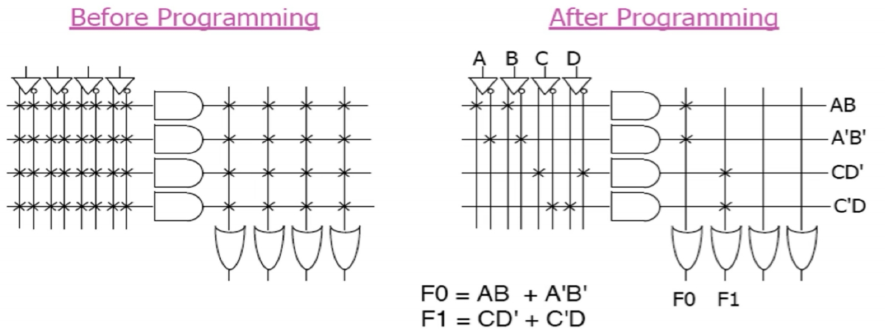
\includegraphics[width=0.86\linewidth]{bf.png}
\end{center}

\noindent Nella figura (a destra, dopo la programmazione) gli incroci segnati con $\times$
sono le connessioni rimaste. Con 4 ingressi $A,B,C,D$ il piano AND genera i 4 implicanti
$AB$, $\overline{A}\,\overline{B}$, $C\overline{D}$, $\overline{C}D$ e il piano OR li combina
nelle due funzioni:
\[
F_0 = AB + \overline{A}\,\overline{B} = \overline{A\oplus B}
\qquad\qquad
F_1 = C\overline{D} + \overline{C}D = C \oplus D
\]

\begin{important}
\textbf{PLA e ROM a confronto.} La ROM genera \emph{tutti} i $2^n$ mintermini e poi sceglie,
nel piano OR, quelli che servono: il piano AND è fisso e cresce esponenzialmente con $n$.
La PLA genera \emph{solo} i prodotti necessari e utili: anche il piano AND è programmabile e
il numero di righe è pari al numero di implicanti distinti (qui 4, contro i $2^4=16$
mintermini che servirebbero a una ROM). Per sfruttarla al meglio le funzioni vanno quindi
prima semplificate (ad esempio con le mappe di Karnaugh, \cref{sec:karnaugh}).
\end{important}

% ======================================================================
\section{Multiplexer e demultiplexer}

\subsection{Multiplexer (MUX)}

\begin{definizione}{MUX}
\textbf{MUX} (\emph{multiplexer}): circuito digitale che funziona similmente a un selettore,
con $2^n$ ingressi di dato, $n$ ingressi di indirizzo (linee di controllo) e 1 uscita.
L'uscita è uguale all'ingresso di dato il cui numero è scritto sugli indirizzi.
\end{definizione}

\noindent Un multiplexer con $2^n$ ingressi e $m$ uscite si indica con $2^n:m$
(ingressi : uscite); il MUX con una sola uscita è quindi un MUX $2^n:1$.

\begin{fitcenter}
\begin{circuitikz}[line width=0.6pt, font=\small, >=latex]
% simbolo generale
\draw[thick, fill=noteblue!4] (0,0) -- (1.2,0.6) -- (1.2,2.4) -- (0,3) -- cycle;
\node at (0.6,1.5) {MUX};
\foreach \y in {2.6,2.1,0.9,0.4}{ \draw[->] (-0.8,\y) -- (0,\y); }
\node at (-0.4,1.55) {$\vdots$};
\node[left, font=\scriptsize, align=right] at (-0.8,1.5) {$2^n$\\ingressi};
\draw[->] (1.2,1.5) -- (2.1,1.5) node[right, font=\scriptsize] {uscita $O$};
\draw[->, very thick] (0.6,-0.9) node[below, font=\scriptsize] {$n$ indirizzi} -- (0.6,0.3);
\node at (3.9,1.5) {$\Longrightarrow$};
% MUX 2:1 a porte
\begin{scope}[xshift=6.2cm]
\node[and port, scale=0.8] (A0) at (3.4,2.4) {};
\node[and port, scale=0.8] (A1) at (3.4,0.6) {};
\node[or port, scale=0.8] (O) at (5.2,1.5) {};
\draw (A0.out) -- ++(0.3,0) |- (O.in 1);
\draw (A1.out) -- ++(0.3,0) |- (O.in 2);
\draw[->] (O.out) -- ++(0.6,0) node[right] {$O$};
\draw (0,0 |- A0.in 1) node[left] {$a_0$} -- (A0.in 1);
\draw (0,0 |- A1.in 1) node[left] {$a_1$} -- (A1.in 1);
\draw (1.2,-0.7) node[below] {$S$} -- (1.2,0 |- A1.in 2) node[circle, fill, inner sep=1pt] {} -- (A1.in 2);
\draw (1.2,0 |- A1.in 2) -- (1.2,0 |- A0.in 2);
\node[not port, scale=0.5, anchor=in 1] (NS) at (1.5,0 |- A0.in 2) {};
\draw (1.2,0 |- A0.in 2) -- (NS.in 1);
\draw (NS.out) -- (A0.in 2);
\node[font=\scriptsize] at (3.4,-0.6) {MUX 2:1 ($n=1$)};
\end{scope}
\end{circuitikz}
\end{fitcenter}

\noindent Per $n=1$ il MUX si realizza con due AND e una OR:
$O = a_0\,\overline{S} + a_1\,S$. Se $S=0$ passa $a_0$, se $S=1$ passa $a_1$. In generale
ogni ingresso $a_k$ entra in una AND insieme al mintermine degli indirizzi che vale $k$, e le
AND sono raccolte da una OR: $O = \sum_k a_k\,m_k(S)$.

\medskip
\begin{important}
\textbf{Ogni funzione a $n$ variabili può essere implementata con un multiplexer
$2^{n-1}:1$.} Si usano $n-1$ variabili come indirizzi; per ogni combinazione degli indirizzi
la funzione, vista come funzione della variabile rimasta, può valere solo $0$, $1$, la
variabile stessa oppure la sua negazione, e questo valore si collega al corrispondente
ingresso di dato.
\end{important}

\noindent Consideriamo $F(a,b,c)=a\overline{b}+abc$ e costruiamo la \textbf{tabella di
verità funzionale} usando $a$ e $b$ come indirizzi di un MUX 4:1 ($2^{3-1}=4$ ingressi):
\begin{itemize}[leftmargin=1.5em, itemsep=1pt]
    \item $ab=00$ e $ab=01$: entrambi i termini contengono $a$, quindi $F=0$;
    \item $ab=10$: il primo termine vale 1, quindi $F=1$ (qualunque sia $c$);
    \item $ab=11$: resta solo il secondo termine, quindi $F=c$.
\end{itemize}

\begin{center}
\begin{minipage}[c]{0.3\linewidth}
\centering
\begin{tabular}{cc|c}
\toprule
$a$ & $b$ & $F$ \\
\midrule
0 & 0 & 0 \\
0 & 1 & 0 \\
1 & 0 & 1 \\
1 & 1 & $c$ \\
\bottomrule
\end{tabular}
\end{minipage}%
\begin{minipage}[c]{0.45\linewidth}
\centering
\begin{tikzpicture}[font=\small, >=latex, line width=0.6pt]
\draw[thick, fill=noteblue!4] (0,0) -- (1.4,0.6) -- (1.4,2.8) -- (0,3.4) -- cycle;
\node at (0.7,1.7) {\footnotesize MUX 4:1};
\foreach \v/\k/\y in {0/00/2.9, 0/01/2.2, 1/10/1.2, c/11/0.5}{
  \draw[->] (-1.0,\y) node[left] {$\v$} -- (0,\y);
  \node[right, font=\tiny] at (0,\y) {\k};
}
\draw[->] (1.4,1.7) -- (2.2,1.7) node[right] {$F$};
\draw[->] (0.45,-0.7) node[below] {$a$} -- (0.45,0.2);
\draw[->] (0.95,-0.7) node[below] {$b$} -- (0.95,0.42);
\end{tikzpicture}
\end{minipage}
\end{center}

\noindent Verifica: $F = \overline{a}\,\overline{b}\cdot 0 + \overline{a}\,b\cdot 0 +
a\,\overline{b}\cdot 1 + a\,b\cdot c = a\overline{b}+abc$.

\subsection{Demultiplexer (DEMUX)}

\begin{definizione}{DEMUX}
\textbf{DEMUX} (\emph{demultiplexer}): circuito digitale opposto al MUX, con 1 ingresso,
$n$ linee di controllo e $2^n$ uscite. L'ingresso viene inviato sull'uscita il cui numero è
scritto sugli indirizzi; tutte le altre uscite valgono 0.
\end{definizione}

\noindent Con la stessa notazione, un demultiplexer si indica con $m:2^n$ (qui $1:2^n$).

\begin{fitcenter}
\begin{circuitikz}[line width=0.6pt, font=\small, >=latex]
\draw[thick, fill=noteblue!4] (0,0.6) -- (1.6,0) -- (1.6,3) -- (0,2.4) -- cycle;
\node at (0.85,1.5) {\scriptsize DEMUX};
\draw[->] (-0.9,1.5) node[left, font=\scriptsize] {ingresso $I$} -- (0,1.5);
\foreach \y in {2.6,2.1,0.9,0.4}{ \draw[->] (1.6,\y) -- (2.4,\y); }
\node at (2.0,1.55) {$\vdots$};
\node[right, font=\scriptsize, align=left] at (2.4,1.5) {$2^n$\\uscite};
\draw[->, very thick] (0.8,-0.9) node[below, font=\scriptsize] {$n$ indirizzi} -- (0.8,0.35);
\node at (4.3,1.5) {$\Longrightarrow$};
\begin{scope}[xshift=6.2cm]
\node[and port, scale=0.8] (A1) at (3.4,2.4) {};
\node[and port, scale=0.8] (A0) at (3.4,0.6) {};
\draw[->] (A1.out) -- ++(0.6,0) node[right] {$o_1$};
\draw[->] (A0.out) -- ++(0.6,0) node[right] {$o_0$};
\draw (0,1.5) node[left] {$I$} -- (0.6,1.5) node[circle, fill, inner sep=1pt] {};
\draw (0.6,1.5) |- (A1.in 1);
\draw (0.6,1.5) |- (A0.in 1);
\draw (1.2,-0.7) node[below] {$S$} -- (1.2,0 |- A1.in 2) -- (A1.in 2);
\node[circle, fill, inner sep=1pt] at (1.2,0 |- A0.in 2) {};
\node[not port, scale=0.5, anchor=in 1] (NS) at (1.5,0 |- A0.in 2) {};
\draw (1.2,0 |- A0.in 2) -- (NS.in 1);
\draw (NS.out) -- (A0.in 2);
\node[font=\scriptsize] at (3.4,-0.6) {DEMUX 1:2 ($n=1$)};
\end{scope}
\end{circuitikz}
\end{fitcenter}

\noindent Per $n=1$: $o_0 = I\,\overline{S}$ e $o_1 = I\,S$. MUX e DEMUX si usano in coppia
per trasmettere più segnali su un'unica linea: il MUX sceglie quale segnale inviare, il DEMUX
all'altra estremità lo smista sull'uscita corretta (gli indirizzi dei due devono essere
sincronizzati).

% ======================================================================
\section{Universal Shift Register (USR)}

\begin{definizione}{USR}
\textbf{USR} (\emph{Universal Shift Register}): dispositivo che permette di inserire i dati in
parallelo o in serie e di spostarli a destra e a sinistra. Riunisce in un unico circuito
tutte le modalità dei registri a scorrimento (SISO, SIPO, PISO, PIPO).
\end{definizione}

\begin{center}
\begin{tikzpicture}[font=\small, >=latex, line width=0.6pt]
\foreach \x/\lab in {0/$n-1$, 2.6/$n$, 5.2/$n+1$}{
  \draw[thick, fill=noteblue!4] (\x,0) rectangle ++(1.6,1.2);
  \node at (\x+0.8,0.6) {\lab};
  \draw[->, green!50!black, thick] (\x+0.55,1.9) -- (\x+0.55,1.2);
  \draw[<-, green!50!black, thick] (\x+1.05,1.9) -- (\x+1.05,1.2);
}
\foreach \x in {-1,1.6,4.2,6.8}{
  \draw[->, red!70!black, thick] (\x,0.85) -- ++(1.0,0);
  \draw[<-, blue!70!black, thick] (\x,0.35) -- ++(1.0,0);
}
\node[font=\scriptsize, green!50!black] at (3.4,2.2) {ingresso / uscita parallela};
\node[font=\scriptsize, red!70!black, right] at (7.9,0.85) {shift right};
\node[font=\scriptsize, blue!70!black, right] at (7.9,0.35) {shift left};
\draw (-1,-0.5) node[left, font=\scriptsize] {$S_1S_0$} -- (6.8,-0.5);
\foreach \x in {0.8,3.4,6.0}{ \draw (\x,-0.5) node[circle, fill, inner sep=1pt] {} -- (\x,0); }
\end{tikzpicture}
\end{center}

\noindent Ogni cella $n$ è un flip-flop D che, a ogni fronte di clock, può caricare uno di
quattro valori: il proprio (hold), quello della cella di sinistra (shift right), quello
della cella di destra (shift left) o il dato parallelo $I_n$. Vediamo come implementare
ogni singola unità dell'USR.

\subsection{La cella elementare}

La scelta fra le quattro funzioni si fa con un \textbf{MUX 4:1}, i cui 2 indirizzi $S_1S_0$
sono comuni a tutte le celle:

\begin{center}
\begin{minipage}[c]{0.36\linewidth}
\centering
\begin{tabular}{cc|l|c}
\toprule
$S_1$ & $S_0$ & funzione & $D_n$ \\
\midrule
0 & 0 & hold & $Q_n$ \\
0 & 1 & shift right & $Q_{n-1}$ \\
1 & 0 & shift left & $Q_{n+1}$ \\
1 & 1 & data in & $I_n$ \\
\bottomrule
\end{tabular}
\end{minipage}%
\hspace{0.2cm}%
\begin{minipage}[c]{0.6\linewidth}
\centering
\begin{circuitikz}[line width=0.6pt, font=\small, >=latex]
\ctikzset{flipflops/scale=0.85}
\draw[thick, fill=noteblue!4] (0,0) -- (1.2,0.6) -- (1.2,2.8) -- (0,3.4) -- cycle;
\node at (0.6,1.7) {\footnotesize MUX};
\foreach \s/\k/\y in {Q_{n-1}/01/2.2, Q_{n+1}/10/1.2, I_n/11/0.5}{
  \draw (-0.9,\y) node[left, font=\scriptsize] {$\s$} -- (0,\y);
  \node[right, font=\tiny] at (0,\y) {\k};
}
\draw[->] (0.4,-0.7) node[below, font=\scriptsize] {$S_1$} -- (0.4,0.2);
\draw[->] (0.85,-0.7) node[below, font=\scriptsize] {$S_0$} -- (0.85,0.42);
\node[and port, scale=0.7] (AN) at (2.5,1.55) {};
\draw (1.2,1.7) -- (1.2,0 |- AN.in 1) -- (AN.in 1);
\node[not port, scale=0.5, rotate=90] (NC) at (1.7,0.5) {};
\draw (1.7,-0.7) node[below, font=\scriptsize] {CLR} -- (NC.in 1);
\draw (NC.out) |- (AN.in 2);
\node[flipflop D] (FF) at (4.3,1.8) {};
\draw (AN.out) -- ++(0.2,0) |- (FF.pin 1) node[above left, font=\scriptsize] {$D_n$};
\draw (FF.pin 3) -- ++(-0.3,0) -- ++(0,-1.6) node[below, font=\scriptsize] {CLK};
\draw[->] (FF.pin 6) -- ++(1.1,0) node[right, font=\scriptsize] {$Q_n$};
\node[right, font=\tiny] at (0,2.9) {00};
\draw (FF.pin 6) ++(0.5,0) node[circle, fill, inner sep=1pt] {} |- (-0.6,3.8) |- (0,2.9);
\node[above, font=\scriptsize] at (1.8,3.8) {$Q_n$ (hold)};
\end{circuitikz}
\end{minipage}
\end{center}

\noindent L'uscita del MUX passa per una porta AND il cui secondo ingresso è
$\overline{\text{CLR}}$: se $\text{CLR}=1$ si ha $D_n=0$ e al fronte di clock successivo il
flip-flop si azzera. Si tratta quindi di un \textbf{reset a 0 sincrono}. Si noti anche il
collegamento $Q_n\to$ ingresso 00, che realizza la funzione di hold.

\subsection{Implementazione a 4 bit}

Collegando quattro celle, l'ingresso 01 (shift right) di ogni cella riceve l'uscita della
cella a sinistra e l'ingresso 10 (shift left) quella della cella a destra. Le celle alle
estremità ricevono invece i due ingressi seriali:
\begin{itemize}[leftmargin=1.5em, itemsep=1pt]
    \item \textbf{RSI} (\emph{Right Serial Input}): entra nella cella $Q_0$ durante lo shift
          right; il dato esce da $Q_3$ (\textbf{RSO}, \emph{Right Serial Output});
    \item \textbf{LSI} (\emph{Left Serial Input}): entra nella cella $Q_3$ durante lo shift
          left; il dato esce da $Q_0$ (\textbf{LSO}, \emph{Left Serial Output}).
\end{itemize}

\begin{fitcenter}
\begin{tikzpicture}[font=\small, >=latex, line width=0.6pt]
\foreach \i in {0,1,2,3}{
  \node[draw, thick, fill=noteblue!4, minimum width=1.9cm, minimum height=1.4cm, align=center]
       (C\i) at (3.2*\i,0) {cella $\i$\\\scriptsize MUX + DFF};
  \draw[->] ($(C\i.north)+(-0.45,0.8)$) node[above] {$I_\i$} -- ($(C\i.north)+(-0.45,0)$);
  \draw[->] ($(C\i.north)+(0.45,0)$) -- ++(0,0.8) node[above] {$Q_\i$};
}
\foreach \i/\j in {0/1, 1/2, 2/3}{
  \draw[->, red!70!black] ($(C\i.east)+(0,0.3)$) -- ($(C\j.west)+(0,0.3)$);
  \draw[<-, blue!70!black] ($(C\i.east)+(0,-0.3)$) -- ($(C\j.west)+(0,-0.3)$);
}
\draw[->, red!70!black] ($(C0.west)+(-1.1,0.3)$) node[left] {RSI} -- ($(C0.west)+(0,0.3)$);
\draw[<-, blue!70!black] ($(C0.west)+(-1.1,-0.3)$) node[left] {LSO} -- ($(C0.west)+(0,-0.3)$);
\draw[->, red!70!black] ($(C3.east)+(0,0.3)$) -- ++(1.1,0) node[right] {RSO};
\draw[<-, blue!70!black] ($(C3.east)+(0,-0.3)$) -- ++(1.1,0) node[right] {LSI};
\foreach \s/\y in {$S_1S_0$/-1.3, CLK/-1.8, CLR/-2.3}{
  \draw (-2.0,\y) node[left, font=\scriptsize] {\s} -- (10.4,\y);
}
\foreach \i in {0,1,2,3}{
  \foreach \dx/\y in {-0.5/-1.3, 0/-1.8, 0.5/-2.3}{
    \draw ($(C\i.south)+(\dx,0)$) -- ($(C\i.south)+(\dx,0)$ |- 0,\y) node[circle, fill, inner sep=1pt] {};
  }
}
\end{tikzpicture}
\end{fitcenter}

\noindent Con lo stesso circuito si ottengono tutte le modalità: caricamento parallelo
($S_1S_0=11$), shift right (01), shift left (10) e hold (00). Ad esempio, per una
trasmissione \textbf{PISO} si carica il dato con $S_1S_0=11$ e poi lo si fa uscire un bit
alla volta con lo shift; per una ricezione \textbf{SIPO} si fanno entrare i bit dall'ingresso
seriale e si leggono le uscite $Q_0\ldots Q_3$.

\subsection{Applicazione: trasmissione seriale Sender--Receiver}

Due USR a 8 bit (ciascuno formato da due integrati a 4 bit in cascata) permettono di
trasmettere un byte su un'unica linea. Il trasmettitore (\emph{Sender}) lavora in modalità
PISO, il ricevitore (\emph{Receiver}) in modalità SIPO; i due condividono il clock.

\begin{fitcenter}
\begin{tikzpicture}[font=\small, >=latex, line width=0.6pt]
\node[draw, thick, fill=noteblue!4, minimum width=3.4cm, minimum height=1.5cm, align=center] (S) at (0,0)
     {\textbf{Sender}\\\scriptsize USR 8 bit (PISO)};
\node[draw, thick, fill=noteblue!4, minimum width=3.4cm, minimum height=1.5cm, align=center] (R) at (7.4,0)
     {\textbf{Receiver}\\\scriptsize USR 8 bit (SIPO)};
\foreach \k in {0,...,7}{
  \draw[->] ($(S.north west)+(0.35+0.385*\k,0.6)$) -- ($(S.north west)+(0.35+0.385*\k,0)$);
  \draw[->] ($(R.north west)+(0.35+0.385*\k,0)$) -- ($(R.north west)+(0.35+0.385*\k,0.6)$);
}
\node[above] at ($(S.north)+(0,0.6)$) {$D_1\ldots D_8$ (dati da trasmettere)};
\node[above] at ($(R.north)+(0,0.6)$) {$D_1\ldots D_8$ (dati ricevuti)};
\draw[->, very thick, notered] (S.east) -- node[above, font=\scriptsize] {linea seriale}
     node[below, font=\scriptsize, black] {LSO $\to$ LSI} (R.west);
\draw (-2.6,-1.4) node[left, font=\scriptsize] {Clock} -- (7.4,-1.4);
\draw[->] (0,-1.4) node[circle, fill, inner sep=1pt] {} -- (S.south);
\draw[->] (7.4,-1.4) -- (R.south);
\draw[->] ($(S.south)+(-1.2,-0.9)$) node[below, font=\scriptsize] {$S_1S_0$} -- ($(S.south)+(-1.2,0)$);
\draw[->] ($(R.south)+(-1.2,-0.9)$) node[below, font=\scriptsize] {$S_1S_0$} -- ($(R.south)+(-1.2,0)$);
\end{tikzpicture}
\end{fitcenter}

\noindent Il flusso dell'operazione è:
\begin{enumerate}[leftmargin=1.8em, itemsep=2pt]
    \item \textbf{caricamento nel Sender} dei dati $D_i$: $S_1S_0=11$ sul Sender, un colpo di
          clock;
    \item \textbf{trasmissione sulla linea seriale}: Sender e Receiver entrambi in shift
          ($S_1S_0=10$); a ogni colpo di clock un bit esce dall'uscita seriale del Sender ed
          entra nell'ingresso seriale del Receiver. Dopo 8 colpi di clock l'intero byte è
          stato trasferito;
    \item \textbf{lettura sulle uscite del Receiver}: il Receiver viene messo in hold
          ($S_1S_0=00$) e i dati $D_1\ldots D_8$ sono disponibili in parallelo.
\end{enumerate}
Il vantaggio è che servono solo una linea dati (più il clock e la massa) invece di otto.

% ======================================================================
\section{Vincoli temporali dell'USR e jitter}

Il clock di un USR non può essere arbitrariamente veloce: fra due fronti consecutivi il
segnale deve uscire da un flip-flop, attraversare il MUX della cella successiva e arrivare
stabile all'ingresso $D$ in tempo per il fronte seguente. La \textbf{massima frequenza del
clock} corrisponde quindi al \textbf{minimo periodo del clock}:

\[
\boxed{T_{\text{CLK,min}} = T_{\text{propag}} + T_{\text{lc}} + T_{\text{setup}} + T_{\text{jitter}}}
\qquad\qquad f_{\text{CLK,max}} = \frac{1}{T_{\text{CLK,min}}}
\]

\begin{itemize}[leftmargin=1.5em, itemsep=1pt]
    \item $T_{\text{propag}}$: ritardo CLK$\to Q$ nel flip-flop;
    \item $T_{\text{lc}}$: ritardo nella logica combinatoria (il MUX e la porta AND);
    \item $T_{\text{setup}}$: tempo per cui $D$ deve restare stabile prima del clock
          successivo;
    \item $T_{\text{jitter}}$: margine per l'incertezza sull'istante di arrivo del fronte.
\end{itemize}

\begin{center}
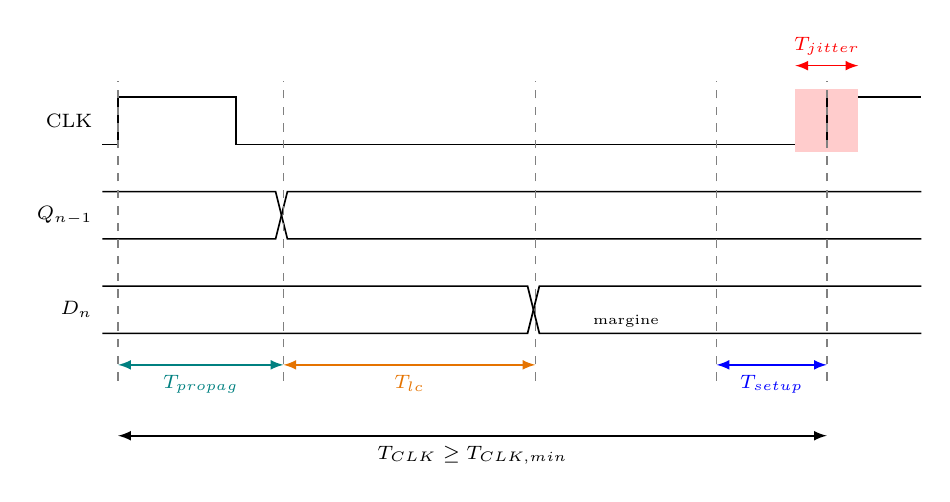
\begin{tikzpicture}[x=1cm, y=1cm, font=\scriptsize, line width=0.6pt, >=latex]
\node[left] at (-0.2,2.3) {CLK};
\draw (-0.2,2) -- (0,2) -- (0,2.6) -- (1.5,2.6) -- (1.5,2) -- (9,2) -- (9,2.6) -- (10.2,2.6);
\fill[red!20] (8.6,1.9) rectangle (9.4,2.7);
\draw (9,2) -- (9,2.6);
\node[left] at (-0.2,1.1) {$Q_{n-1}$};
\draw (-0.2,0.8) -- (2,0.8) -- (2.15,1.4) -- (10.2,1.4);
\draw (-0.2,1.4) -- (2,1.4) -- (2.15,0.8) -- (10.2,0.8);
\node[left] at (-0.2,-0.1) {$D_n$};
\draw (-0.2,-0.4) -- (5.2,-0.4) -- (5.35,0.2) -- (10.2,0.2);
\draw (-0.2,0.2) -- (5.2,0.2) -- (5.35,-0.4) -- (10.2,-0.4);
\foreach \x in {0,2.1,5.3,7.6,9}{ \draw[dashed, gray] (\x,-1.0) -- (\x,2.8); }
\draw[<->, teal] (0,-0.8) -- node[below] {$T_{\text{propag}}$} (2.1,-0.8);
\draw[<->, orange!90!black] (2.1,-0.8) -- node[below] {$T_{\text{lc}}$} (5.3,-0.8);
\draw[<->, blue] (7.6,-0.8) -- node[below] {$T_{\text{setup}}$} (9,-0.8);
\draw[<->, red] (8.6,3.0) -- node[above] {$T_{\text{jitter}}$} (9.4,3.0);
\draw[<->] (0,-1.7) -- node[below] {$T_{\text{CLK}} \ge T_{\text{CLK,min}}$} (9,-1.7);
\node[align=center] at (6.45,-0.25) {\tiny margine};
\end{tikzpicture}
\end{center}

\begin{definizione}{Jitter del CLK}
$\Delta_{\max}$ fra gli istanti di arrivo dei fronti di clock che dovrebbero giungere
\emph{contemporaneamente} a tutti i componenti del circuito, ma che in pratica non lo fanno a
causa di variazioni fisiche (diversa lunghezza dei percorsi, carichi diversi, rumore,
variazioni di temperatura).
\end{definizione}

\noindent Se il fronte arriva alla cella successiva in anticipo rispetto a quello della cella
precedente, il tempo disponibile si riduce: per questo il jitter va sommato agli altri
ritardi nel calcolo di $T_{\text{CLK,min}}$.

% ======================================================================
\section*{Riepilogo del Capitolo}

\begin{important}
Blocchi combinatori di alto livello (\textbf{ROM, PLA, MUX, DEMUX}) permettono di implementare funzioni logiche complesse senza progettare reti di porte su misura, e si combinano con i Flip-Flop per costruire registri evoluti come l'USR, il cui limite di velocità è fissato dalla somma dei ritardi di propagazione, logica, setup e jitter.
\end{important}

\begin{note}
\textbf{Formule fondamentali:}
\begin{itemize}
    \item \textbf{ROM:} $n$ ingressi $\to 2^n$ parole di $p$ bit; equivale a un decoder (piano AND, genera i mintermini) seguito da un encoder (piano OR).
    \item \textbf{Multiplexer generico:} $O = \sum_k a_k\, m_k(S)$; teorema del MUX: ogni funzione a $n$ variabili è implementabile con un multiplexer $2^{n-1}{:}1$.
    \item \textbf{Demultiplexer ($n=1$):} $o_0 = I\overline{S}$, $\; o_1 = IS$.
    \item \textbf{Cella USR:} MUX $4{:}1$ (hold / shift-right / shift-left / data-in) seguito da un Flip-Flop D con reset sincrono.
    \item \textbf{Vincolo temporale:} $T_{\text{CLK,min}} = T_{\text{propag}} + T_{\text{lc}} + T_{\text{setup}} + T_{\text{jitter}}$, $\; f_{\text{CLK,max}} = 1/T_{\text{CLK,min}}$.
\end{itemize}
\end{note}

